\documentclass[aspectratio=169,11pt]{beamer}
\usepackage[T1]{fontenc}
\usepackage[utf8]{inputenc}
\usepackage[french]{babel}
\usepackage{lmodern}
\usepackage{booktabs}
\usepackage{tabularx}
\usepackage{tikz}
\usepackage{fontawesome5}
\usetikzlibrary{positioning,arrows.meta,calc,fit}

\usetheme[progressbar=frametitle,numbering=fraction]{metropolis}

\definecolor{nuit}{HTML}{14213D}
\definecolor{papier}{HTML}{F7F6F2}
\definecolor{bleu}{HTML}{1F5FAD}
\definecolor{bleuclair}{HTML}{DCE7F6}
\definecolor{orange}{HTML}{C2581F}
\definecolor{orangeclair}{HTML}{F6E6DA}
\definecolor{vert}{HTML}{2E7D32}
\definecolor{gris}{HTML}{4A5568}
\definecolor{trait}{HTML}{DDD8CC}

\setbeamercolor{normal text}{fg=nuit,bg=papier}
\setbeamercolor{frametitle}{fg=papier,bg=nuit}
\setbeamercolor{progress bar}{fg=bleu,bg=bleuclair}
\setbeamercolor{alerted text}{fg=orange}
\setbeamercolor{title separator}{fg=bleu}
\setbeamercolor{background canvas}{bg=papier}

\tikzset{
  carte/.style={draw=trait,fill=white,rounded corners=4pt,align=center,inner sep=6pt,font=\small,execute at begin node={\hyphenpenalty=10000}},
  fleche/.style={-{Stealth[length=2.5mm]},thick,bleu},
}

\title{Dessiner un graphe directement en espace écran}
\subtitle{Jalon 1 : où en est le projet}
\author{Melissa Colin \and Quentin Lopez \and Yani Haouchine}
\institute{ENSEIRB-MATMECA 3A, projet semestriel \quad·\quad Encadrant : Romain Giot (LaBRI)}
\date{6 novembre 2026}

\begin{document}

\maketitle

%---------------------------------------------------------------------
\begin{frame}{Plan}
\begin{enumerate}
\setlength{\itemsep}{6pt}
\item Le sujet en une slide
\item Un rapide état de l'art
\item Notre idée générale
\item Premiers choix techniques : les données, l'architecture, la loss
\item Premiers résultats
\item Idées pour la suite
\end{enumerate}
\end{frame}

%---------------------------------------------------------------------
\begin{frame}{Le sujet}
\centering
\textbf{Optimiser la position des nœuds d'un graphe directement en espace écran,}\\\textbf{avec des coûts calculés sur le dessin rendu en pixels.}

\vspace{0.6cm}
\begin{tikzpicture}[node distance=0.5cm]
  \node[carte,text width=4.0cm] (e) {\textcolor{bleu}{\scriptsize ENTRÉE}\\\textbf{Un graphe}\\[2pt]\scriptsize arêtes, taille des nœuds, en option largeur des arêtes et couleurs};
  \node[carte,text width=4.0cm,right=of e] (s) {\textcolor{bleu}{\scriptsize SORTIE}\\\textbf{Des positions}\\[2pt]\scriptsize $(x, y)$ pour chaque nœud, et éventuellement l'image};
  \node[carte,text width=4.0cm,right=of s] (c) {\textcolor{orange}{\scriptsize MOYEN}\\\textbf{Un rendu différentiable}\\[2pt]\scriptsize nœuds et arêtes dessinés avec des SDF, d'où des coûts écran dérivables};
\end{tikzpicture}

\vspace{0.5cm}
\small Question centrale du sujet : des coûts définis à l'écran donnent-ils des dessins plus fidèles au rendu final que des coûts géométriques ?
\end{frame}

%---------------------------------------------------------------------
\begin{frame}{Un rapide état de l'art}
\small
\begin{tabularx}{\textwidth}{@{}l X@{}}
\toprule
\textbf{Méthode} & \textbf{Principe} \\
\midrule
Kamada-Kawai, stress & optimisation classique, refaite pour chaque graphe \\
(GD)$^2$ & descente de gradient sur des critères esthétiques, graphe par graphe \\
DeepGD & un GNN appris une fois, entraîné sur le stress \\
SmartGD & un GAN qui imite des dessins de référence \\
CoRe-GD (ICLR 2024) & un GNN récurrent qui se recâble selon son propre dessin ; meilleur stress sur Rome \\
\bottomrule
\end{tabularx}

\vspace{0.5cm}
\textcolor{gris}{Toutes optimisent dans un espace géométrique, où un nœud est un point et une arête un segment sans épaisseur. Les pixels n'arrivent qu'à l'affichage.}
\end{frame}

%---------------------------------------------------------------------
\begin{frame}{Notre idée : un réseau qui place les nœuds directement en pixels}
\centering
\begin{tikzpicture}[node distance=0.32cm]
  \node[carte] (g) {\textbf{Graphe}\\\scriptsize nœuds, arêtes, tailles};
  \node[carte,right=of g,fill=bleuclair,draw=bleu] (gnn) {\textbf{Modèle}\\\scriptsize GNN};
  \node[carte,right=of gnn] (pos) {\textbf{Positions}\\\scriptsize $(N,2)$ en pixels};
  \node[carte,right=of pos,fill=orangeclair,draw=orange] (cout) {\textbf{Loss}\\\scriptsize métriques visuelles};
  \draw[fleche] (g) -- (gnn);
  \draw[fleche] (gnn) -- (pos);
  \draw[fleche] (pos) -- (cout);
  \draw[-{Stealth[length=2.5mm]},thick,orange,dashed] (cout.south) -- ++(0,-0.55) -| node[pos=0.25,below,font=\scriptsize]{le gradient remonte jusqu'aux poids du modèle} (gnn.south);
\end{tikzpicture}

\vspace{0.6cm}
\begin{minipage}{0.86\textwidth}
\small Les trois axes du sujet, et où nous en sommes :
\begin{itemize}
\setlength{\itemsep}{2pt}
\item des coûts calculés à l'écran : en cours, c'est notre loss ;
\item l'optimisation directe, graphe par graphe : pas encore commencée ;
\item un modèle appris sur la base Rome : notre point de départ, sans dessins de référence puisque la loss note le dessin produit.
\end{itemize}
\end{minipage}
\end{frame}

%---------------------------------------------------------------------
\begin{frame}{Les données}
\begin{columns}[T]
\begin{column}{0.48\textwidth}
\begin{block}{Base Rome}
\small 11\,534 graphes de 10 à 110 nœuds.\\
Découpage fixe : 70\,\% entraînement, 10\,\% validation, 20\,\% test.
\end{block}
\end{column}
\begin{column}{0.48\textwidth}
\begin{block}{Ce que le modèle voit d'un nœud}
\small Son degré, un bruit aléatoire et 8 encodages de position (vecteurs propres du Laplacien), plus les distances dans le graphe pour la loss.
\end{block}
\end{column}
\end{columns}

\vspace{0.4cm}
\small Format PyTorch Geometric : plusieurs graphes traités en un seul batch, entraînement sur GPU.

\vspace{0.4cm}
\begin{tikzpicture}
  \node[carte,draw=orange,fill=orangeclair,text width=0.9\textwidth,align=left] {\textcolor{orange}{\large\faLightbulb[regular]}\quad\small La loss n'a pas besoin de dessins de référence. On pourrait donc générer des graphes aléatoires à volonté, au lieu de dépendre de la base Rome.};
\end{tikzpicture}
\end{frame}

%---------------------------------------------------------------------
\begin{frame}{L'architecture : un GNN récurrent et une sortie en pixels}
\centering
\begin{tikzpicture}[node distance=0.35cm]
  \node[carte] (enc) {\textbf{Encodeur}\\\scriptsize un MLP par nœud};
  \node[carte,right=0.7cm of enc] (mp) {\textbf{Messages}\\\scriptsize le long des arêtes};
  \node[carte,right=of mp] (br) {\textbf{Brouillon}\\\scriptsize de dessin};
  \node[carte,right=of br] (knn) {\textbf{Messages}\\\scriptsize entre voisins\\[-2pt]\scriptsize dans le dessin};
  \node[carte,right=0.7cm of knn,fill=bleuclair,draw=bleu] (sa) {\textbf{Soft-argmax}\\\scriptsize positions en pixels};
  \node[draw=bleu,dashed,rounded corners=6pt,fit=(mp)(br)(knn),inner sep=7pt,label={[font=\scriptsize,bleu]above:répété environ 5 fois}] (boucle) {};
  \draw[fleche] (enc) -- (boucle);
  \draw[fleche] (mp) -- (br);
  \draw[fleche] (br) -- (knn);
  \draw[fleche] (boucle) -- (sa);
\end{tikzpicture}

\vspace{0.6cm}
\small
\begin{itemize}
\item Boucle reprise de CoRe-GD : deux nœuds proches dans le dessin échangent des messages, et peuvent apprendre à s'écarter.
\item Soft-argmax en sortie : la position est la moyenne d'une carte de probabilités sur les pixels, donc toujours dans le cadre (slide suivante).
\end{itemize}
\end{frame}

%---------------------------------------------------------------------
\begin{frame}{Soft-argmax : une sortie dans l'espace des pixels}
\centering
\begin{tikzpicture}
  % ---------------- gauche : origine, estimation de pose humaine
  \node[font=\footnotesize\bfseries] at (1.6,3.35) {Origine : la pose humaine};
  \begin{scope}[shift={(1.2,0.25)},line width=1.6pt,nuit,line cap=round]
    \draw (0,2.25) circle (0.25);
    \draw (0,2.0) -- (0,1.0);
    \draw (0,1.75) -- (-0.45,1.25) -- (-0.65,0.75);
    \draw (0,1.75) -- (0.5,1.35) -- (0.85,1.7);
    \draw (0,1.0) -- (-0.35,0.15);
    \draw (0,1.0) -- (0.35,0.15);
    \fill[orange!18] (0.85,1.7) circle (0.42);
    \fill[orange!40] (0.85,1.7) circle (0.26);
    \fill[orange!85] (0.85,1.7) circle (0.1);
  \end{scope}
  \draw[-{Stealth[length=2mm]},thick,orange] (2.35,1.95) -- (3.0,1.95) node[right,font=\scriptsize,nuit,align=left] {$(x, y)$\\du poignet};
  \node[font=\scriptsize,gris,align=center] at (1.6,-0.4) {carte de chaleur d'une articulation\\$\rightarrow$ sa position dans l'image};

  % ---------------- séparation
  \draw[trait,thick] (4.25,-0.4) -- (4.25,3.5);

  % ---------------- droite : chez nous, un nœud
  \node[font=\footnotesize\bfseries] at (7.6,3.35) {Chez nous : un nœud du graphe};
  \begin{scope}[shift={(5.1,0.15)},scale=0.36]
    \foreach \i in {0,...,7} {
      \foreach \j in {0,...,7} {
        \pgfmathsetmacro{\v}{90*exp(-((\i-4.4)^2+(\j-3.3)^2)/2.6)}
        \fill[bleu!\v!white] (\i,\j) rectangle ++(1,1);
      }
    }
    \draw[step=1,trait] (0,0) grid (8,8);
    % position moyenne (continue, entre deux cases)
    \fill[orange] (4.95,3.85) circle (0.28);
    \draw[orange,thick] (4.95,3.85) circle (0.5);
  \end{scope}
  \draw[-{Stealth[length=2mm]},thick,orange] (7.2,1.55) -- (8.25,1.55) node[right,font=\scriptsize,nuit,align=left] {position $(x, y)$\\continue,\\entre deux pixels};
  \node[font=\scriptsize,gris,align=center] at (6.55,-0.4) {probabilité par pixel\\(softmax)};

  % ---------------- formule
  \node[font=\small] at (4.55,-1.35) {$\displaystyle (x, y) \;=\; \sum_{\text{pixels } p} \mathrm{softmax}(s)_p \cdot \mathrm{coord}(p)$};
  \node[font=\scriptsize,gris] at (4.55,-1.95) {moyenne pondérée : différentiable, contrairement à argmax};
  \node[font=\tiny,gris] at (4.55,-2.35) {Integral Pose Regression (Sun et al., 2018) \quad·\quad DSNT (Nibali et al., 2018)};
\end{tikzpicture}
\end{frame}

%---------------------------------------------------------------------
\begin{frame}{La loss : les métriques de la littérature}
\small La loss est une somme pondérée de métriques différentiables : $\mathcal{L} = \sum_k w_k \, m_k$. Nous avons d'abord trié les métriques existantes.

\vspace{0.4cm}
\centering
\begin{tikzpicture}[
  puce/.style={draw=trait,fill=white,rounded corners=3pt,minimum height=0.6cm,text width=6.1cm,align=left,inner sep=4pt},
]
  \node[font=\small\bfseries,bleu] at (0,3.75) {À conserver ou adapter};
  \node[puce] at (0,3.1) {\footnotesize\textbf{Stress de Kamada-Kawai}\hfill\scriptsize\textcolor{gris}{distances}};
  \node[puce] at (0,2.4) {\footnotesize\textbf{Aspect ratio}\hfill\scriptsize\textcolor{gris}{proche d'un carré}};
  \node[puce] at (0,1.7) {\footnotesize\textbf{Angular resolution}\hfill\scriptsize\textcolor{gris}{pas d'angle trop petit}};
  \node[puce] at (0,1.0) {\footnotesize\textbf{Edge crossings}\hfill\scriptsize\textcolor{gris}{moins de croisements}};
  \node[font=\small\bfseries,gris] at (7.1,3.75) {Non essentiel pour nous};
  \node[puce] at (7.1,3.1) {\footnotesize\textcolor{gris}{\textbf{Cluster overlap}}\hfill\scriptsize\textcolor{gris}{séparer les clusters}};
  \node[puce] at (7.1,2.4) {\footnotesize\textcolor{gris}{\textbf{Neighborhood preservation}}\hfill\scriptsize\textcolor{gris}{voisins conservés}};
  \draw[bleu,line width=1.2pt] (-3.35,0.65) -- (-3.35,3.45);
  \draw[trait,line width=1.2pt] (3.75,2.05) -- (3.75,3.45);
\end{tikzpicture}

\end{frame}

%---------------------------------------------------------------------
\begin{frame}{La loss : les métriques choisies pour les nœuds}
\begin{columns}[T]
%--- Stress
\begin{column}{0.32\textwidth}
\centering
\textbf{Stress}\\[4pt]
\begin{tikzpicture}[scale=0.85,nd/.style={circle,fill=bleu,inner sep=1.6pt}]
  \node[nd,label={[font=\scriptsize]left:$u$}] (u) at (0,0) {};
  \node[nd] (a) at (0.7,1.1) {};
  \node[nd] (b) at (1.7,1.25) {};
  \node[nd,label={[font=\scriptsize]right:$v$}] (v) at (2.4,0.1) {};
  \draw[gris,thick] (u) -- (a) -- (b) -- (v);
  \draw[orange,thick,dashed] (u) -- (v);
  \node[font=\scriptsize,orange] at (1.2,-0.4) {distance dessinée};
  \node[font=\scriptsize,gris] at (1.2,1.65) {$d_G(u,v) = 3$ arêtes};
\end{tikzpicture}\\[4pt]
\scriptsize $\displaystyle\sum_{u<v} \frac{(\|p_u - p_v\| - d_{uv})^2}{d_{uv}^2}$\\[4pt]
\textcolor{gris}{respecter la structure du graphe}
\end{column}
%--- Screen
\begin{column}{0.32\textwidth}
\centering
\textbf{Écran}\\[4pt]
\begin{tikzpicture}[scale=0.85]
  \draw[nuit,thick] (0,0) rectangle (2.8,1.8);
  \foreach \p in {(0.9,0.6),(1.2,1.0),(1.5,0.7),(1.7,1.15),(1.95,0.55),(1.1,0.45)} \fill[bleu] \p circle (1.6pt);
  \draw[bleu,dashed] (0.9,0.45) rectangle (1.95,1.15);
  \draw[orange,{Stealth[length=1.5mm]}-{Stealth[length=1.5mm]}] (0,0.25) -- (0.9,0.25);
  \draw[orange,{Stealth[length=1.5mm]}-{Stealth[length=1.5mm]}] (1.95,0.25) -- (2.8,0.25);
  \draw[orange,{Stealth[length=1.5mm]}-{Stealth[length=1.5mm]}] (2.4,1.15) -- (2.4,1.8);
  \node[font=\scriptsize,gris] at (1.4,-0.25) {cadre $W \times H$};
\end{tikzpicture}\\[4pt]
\scriptsize $\displaystyle 2 - \frac{\Delta x}{W} - \frac{\Delta y}{H}$\\[4pt]
\textcolor{gris}{occuper tout le cadre (inspirée de l'aspect ratio)}
\end{column}
%--- Node overlaps
\begin{column}{0.32\textwidth}
\centering
\textbf{Chevauchement}\\[4pt]
\begin{tikzpicture}[scale=0.85]
  \fill[bleuclair] (0.6,0.6) rectangle ++(0.2,0.2);
  \fill[bleuclair] (0.6,0.8) rectangle ++(0.2,0.2);
  \fill[bleuclair] (0.6,1.0) rectangle ++(0.2,0.2);
  \fill[bleuclair] (0.6,1.2) rectangle ++(0.2,0.2);
  \fill[bleuclair] (0.8,0.4) rectangle ++(0.2,0.2);
  \fill[bleuclair] (0.8,0.6) rectangle ++(0.2,0.2);
  \fill[bleuclair] (0.8,0.8) rectangle ++(0.2,0.2);
  \fill[bleuclair] (0.8,1.0) rectangle ++(0.2,0.2);
  \fill[bleuclair] (0.8,1.2) rectangle ++(0.2,0.2);
  \fill[bleuclair] (0.8,1.4) rectangle ++(0.2,0.2);
  \fill[bleuclair] (1.0,0.4) rectangle ++(0.2,0.2);
  \fill[bleuclair] (1.0,0.6) rectangle ++(0.2,0.2);
  \fill[bleuclair] (1.0,0.8) rectangle ++(0.2,0.2);
  \fill[bleuclair] (1.0,1.0) rectangle ++(0.2,0.2);
  \fill[bleuclair] (1.0,1.2) rectangle ++(0.2,0.2);
  \fill[bleuclair] (1.0,1.4) rectangle ++(0.2,0.2);
  \fill[bleuclair] (1.2,0.4) rectangle ++(0.2,0.2);
  \fill[bleuclair] (1.2,0.6) rectangle ++(0.2,0.2);
  \fill[bleuclair] (1.2,0.8) rectangle ++(0.2,0.2);
  \fill[bleuclair] (1.2,1.0) rectangle ++(0.2,0.2);
  \fill[bleuclair] (1.2,1.2) rectangle ++(0.2,0.2);
  \fill[bleuclair] (1.2,1.4) rectangle ++(0.2,0.2);
  \fill[bleuclair] (1.4,0.4) rectangle ++(0.2,0.2);
  \fill[orange] (1.4,0.6) rectangle ++(0.2,0.2);
  \fill[orange] (1.4,0.8) rectangle ++(0.2,0.2);
  \fill[orange] (1.4,1.0) rectangle ++(0.2,0.2);
  \fill[orange] (1.4,1.2) rectangle ++(0.2,0.2);
  \fill[bleuclair] (1.6,0.4) rectangle ++(0.2,0.2);
  \fill[orange] (1.6,0.6) rectangle ++(0.2,0.2);
  \fill[orange] (1.6,0.8) rectangle ++(0.2,0.2);
  \fill[orange] (1.6,1.0) rectangle ++(0.2,0.2);
  \fill[bleuclair] (1.6,1.2) rectangle ++(0.2,0.2);
  \fill[bleuclair] (1.6,1.4) rectangle ++(0.2,0.2);
  \fill[bleuclair] (1.8,0.4) rectangle ++(0.2,0.2);
  \fill[bleuclair] (1.8,0.6) rectangle ++(0.2,0.2);
  \fill[bleuclair] (1.8,0.8) rectangle ++(0.2,0.2);
  \fill[bleuclair] (1.8,1.0) rectangle ++(0.2,0.2);
  \fill[bleuclair] (1.8,1.2) rectangle ++(0.2,0.2);
  \fill[bleuclair] (1.8,1.4) rectangle ++(0.2,0.2);
  \fill[bleuclair] (2.0,0.4) rectangle ++(0.2,0.2);
  \fill[bleuclair] (2.0,0.6) rectangle ++(0.2,0.2);
  \fill[bleuclair] (2.0,0.8) rectangle ++(0.2,0.2);
  \fill[bleuclair] (2.0,1.0) rectangle ++(0.2,0.2);
  \fill[bleuclair] (2.0,1.2) rectangle ++(0.2,0.2);
  \fill[bleuclair] (2.0,1.4) rectangle ++(0.2,0.2);
  \fill[bleuclair] (2.2,0.4) rectangle ++(0.2,0.2);
  \fill[bleuclair] (2.2,0.6) rectangle ++(0.2,0.2);
  \fill[bleuclair] (2.2,0.8) rectangle ++(0.2,0.2);
  \fill[bleuclair] (2.2,1.0) rectangle ++(0.2,0.2);
  \fill[bleuclair] (2.2,1.2) rectangle ++(0.2,0.2);
  \fill[bleuclair] (2.4,0.6) rectangle ++(0.2,0.2);
  \fill[bleuclair] (2.4,0.8) rectangle ++(0.2,0.2);
  \fill[bleuclair] (2.4,1.0) rectangle ++(0.2,0.2);
  \draw[step=0.2,trait,very thin] (0,0) grid (2.8,1.8);
  \draw[bleu,thick] (1.15,0.95) circle (0.62);
  \draw[bleu,thick] (1.95,0.95) circle (0.62);
  \node[font=\scriptsize,gris] at (1.4,-0.25) {pixels dans les deux disques};
\end{tikzpicture}\\[4pt]
\scriptsize $\displaystyle\sum_{\text{pixels}} \sigma\!\Big(\tfrac{-\mathrm{SDF}_i}{s}\Big)\,\sigma\!\Big(\tfrac{-\mathrm{SDF}_j}{s}\Big)$\\[4pt]
\textcolor{gris}{des nœuds, pixel par pixel avec des SDF}
\end{column}
\end{columns}

\vspace{0.35cm}
\centering\scriptsize\textcolor{gris}{Prochaine étape : mettre le stress à l'échelle des pixels, il compte aujourd'hui une arête pour un pixel.}
\end{frame}

%---------------------------------------------------------------------
\begin{frame}{La loss : les métriques pour les arêtes, en cours}
\begin{columns}[T]
\begin{column}{0.45\textwidth}
\centering
\textbf{Chevauchement des arêtes}\\[6pt]
\begin{tikzpicture}[scale=0.9]
  \begin{scope}
    \clip (0.15,0.2) -- (2.85,1.4) -- (2.75,1.62) -- (0.05,0.42) -- cycle;
    \fill[orange] (0.3,1.55) -- (2.7,0.25) -- (2.82,0.47) -- (0.42,1.77) -- cycle;
  \end{scope}
  \draw[bleu,thick,fill=bleuclair,fill opacity=0.6] (0.15,0.2) -- (2.85,1.4) -- (2.75,1.62) -- (0.05,0.42) -- cycle;
  \draw[bleu,thick,fill=bleuclair,fill opacity=0.6] (0.3,1.55) -- (2.7,0.25) -- (2.82,0.47) -- (0.42,1.77) -- cycle;
  \begin{scope}
    \clip (0.15,0.2) -- (2.85,1.4) -- (2.75,1.62) -- (0.05,0.42) -- cycle;
    \fill[orange] (0.3,1.55) -- (2.7,0.25) -- (2.82,0.47) -- (0.42,1.77) -- cycle;
  \end{scope}
\end{tikzpicture}\\[6pt]
\footnotesize Pénalise la zone où deux arêtes épaisses se recouvrent, avec des SDF.\\
\textcolor{gris}{inspirée du nombre de croisements}
\end{column}
\begin{column}{0.45\textwidth}
\centering
\textbf{Angles entre arêtes}\\[6pt]
\begin{tikzpicture}[scale=0.9]
  \coordinate (o) at (1.2,0.5);
  \draw[gris,thick] (o) -- ++(15:1.5);
  \draw[gris,thick] (o) -- ++(40:1.5);
  \draw[gris,thick] (o) -- ++(150:1.3);
  \draw[orange,thick] (o) ++(15:0.75) arc (15:40:0.75);
  \node[font=\scriptsize,orange] at ($(o)+(27:1.95)$) {$\theta_{\min}$};
  \fill[bleu] (o) circle (2.2pt);
\end{tikzpicture}\\[6pt]
\footnotesize Éviter les angles trop petits entre arêtes d'un même nœud.\\
\textcolor{gris}{reprendre l'angular resolution telle quelle ? à décider}
\end{column}
\end{columns}
\end{frame}

%---------------------------------------------------------------------
\begin{frame}{Premiers résultats : comparaison avec l'état de l'art}
\begin{columns}[c]
\begin{column}{0.40\textwidth}
\centering
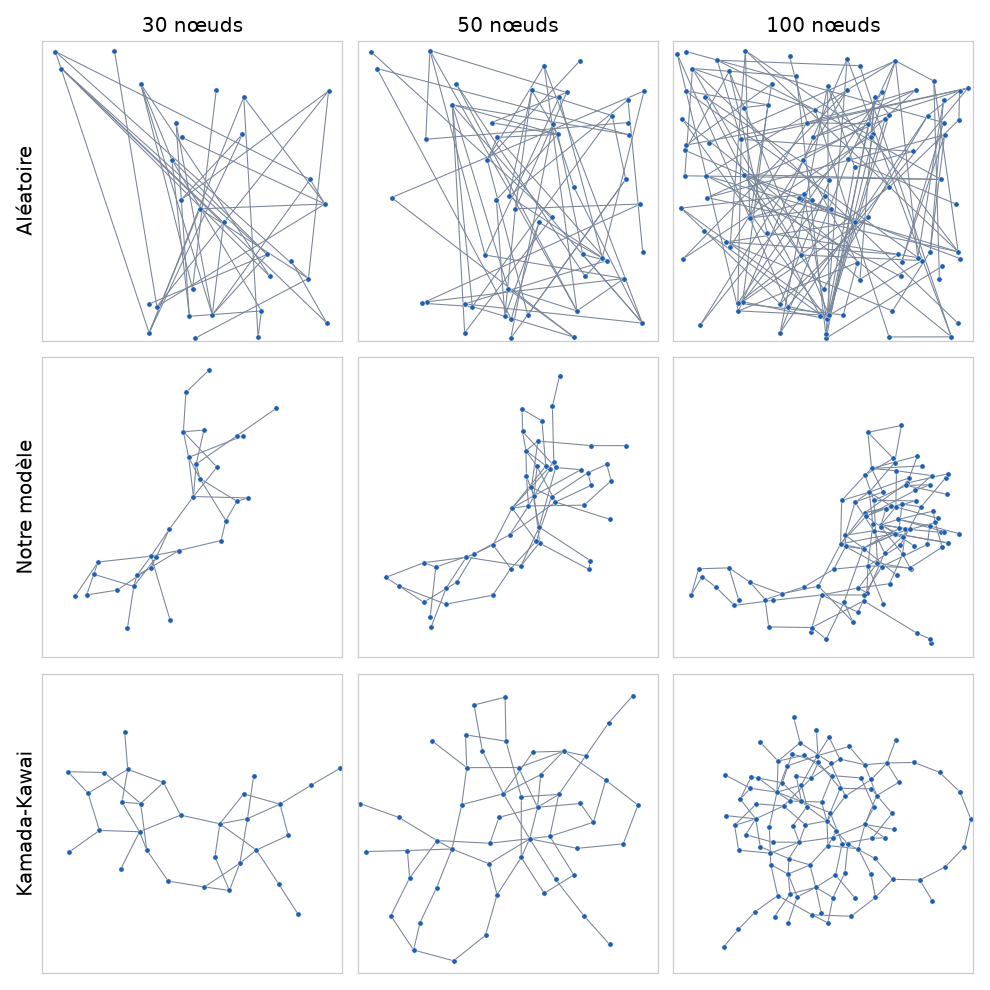
\includegraphics[height=0.7\textheight]{resultats.png}
\end{column}
\begin{column}{0.58\textwidth}
\footnotesize
\setlength{\tabcolsep}{4pt}
\begin{tabular}{@{}lccc@{}}
\toprule
 & \textbf{Stress} & \textbf{Croisements} & \textbf{Nœuds} \\
 & \textbf{normalisé} $\downarrow$ & \textbf{d'arêtes} $\downarrow$ & \textbf{superposés} $\downarrow$ \\
\midrule
Aléatoire & 0,420 & 615 & 0,07\,\% \\
Notre modèle & 0,140 & 77 & 0,33\,\% \\
\midrule
Kamada-Kawai & 0,062 & 30 & \textbf{0\,\%} \\
DeepGD & 0,060 & 30 & 0,02\,\% \\
CoRe-GD & \textbf{0,059} & \textbf{29} & \textbf{0\,\%} \\
\bottomrule
\end{tabular}

\vspace{2pt}
{\scriptsize\textcolor{gris}{204 graphes de Rome jamais vus à l'entraînement.}}
\end{column}
\end{columns}
\end{frame}

%---------------------------------------------------------------------
\begin{frame}{Suite : d'ici le jalon 2}
\begin{enumerate}
\setlength{\itemsep}{7pt}
\item Entraîner le modèle avec la loss commune, le stress mis à l'échelle des pixels
\item Ajouter les métriques sur les arêtes (chevauchements, angles)
\item Faire occuper tout le cadre aux dessins, qui restent souvent dans un coin
\item Stabiliser l'entraînement, dont la validation varie beaucoup d'une epoch à l'autre
\item Comparer aléatoire, Kamada-Kawai, méthodes apprises et notre modèle sur les mêmes métriques
\end{enumerate}
\end{frame}

%---------------------------------------------------------------------
\begin{frame}{Suite : alléger la sortie soft-argmax}
\small Aujourd'hui : 250\,000 scores par nœud (une carte $500 \times 500$), donc 4 graphes par batch au plus sur notre GPU.

\vspace{0.4cm}
\centering
\begin{tikzpicture}[node distance=0.4cm]
  \node[carte,text width=2.6cm,draw=bleu,line width=0.8pt] (a) {\textbf{Tête séparable}\\[2pt]\scriptsize 500 scores pour $x$, 500 pour $y$ : même position, 250 fois moins de mémoire};
  \node[carte,text width=2.6cm,right=of a] (b) {\textbf{Grille plus grossière}\\[2pt]\scriptsize $100 \times 100$ : la position reste continue};
  \node[carte,text width=2.6cm,right=of b] (c) {\textbf{Précision mixte}\\[2pt]\scriptsize calculs en 16 bits};
  \node[carte,text width=2.6cm,right=of c] (d) {\textbf{Accumulation}\\[2pt]\scriptsize simuler un batch de 16 avec $4 \times 4$};
\end{tikzpicture}
\end{frame}

%---------------------------------------------------------------------
\begin{frame}{Suite : une taille d'image variable}
\small Aujourd'hui, la taille de l'image est figée dans les poids : la tête a exactement $W \times H$ sorties.

\vspace{0.3cm}
\begin{columns}[T]
\begin{column}{0.48\textwidth}
\begin{block}{Grille normalisée}
\small Le modèle dessine dans $[0,1]^2$, puis on convertit en pixels à la sortie :\\
$x_{\text{px}} = m + x \cdot (W - 2m)$.\\
La taille de l'image devient une entrée, plus un hyperparamètre.
\end{block}
\end{column}
\begin{column}{0.48\textwidth}
\begin{block}{Dire au modèle pour quelle image il dessine}
\small Lui donner le rapport $W/H$ et la taille des nœuds rapportée à l'image ($r/W$), et tirer des tailles d'image variées pendant l'entraînement.
\end{block}
\end{column}
\end{columns}

\vspace{0.3cm}
\scriptsize\textcolor{gris}{Option plus ambitieuse : un réseau qui donne un score pour n'importe quel point $(x, y)$, évalué sur la grille voulue. Plus souple, mais il faut un calcul par nœud et par pixel.}
\end{frame}

%---------------------------------------------------------------------
\begin{frame}{Suite : rendre le modèle attentif aux arêtes}
\small Les arêtes ne sont pas prédites, ce sont des segments entre les nœuds. Pourtant, la plupart des défauts à l'écran viennent d'elles.

\vspace{0.3cm}
\begin{columns}[T]
\begin{column}{0.48\textwidth}
\begin{block}{A. Tête auxiliaire}
\small Une tête en plus prédit les défauts de chaque arête (croisements, nœud caché, longueur). Entraînée par une perte auxiliaire, elle force le modèle à encoder l'information sur les arêtes.
\end{block}
\end{column}
\begin{column}{0.48\textwidth}
\begin{block}{B. Raffinement itératif}
\small Une première passe propose des positions. On calcule exactement les défauts de chaque arête, puis une seconde passe les reçoit en entrée et corrige.
\end{block}
\end{column}
\end{columns}
\end{frame}

%---------------------------------------------------------------------
\begin{frame}{Bonus : affiner le modèle selon nos préférences}
\small On annote des paires de dessins (\og je préfère A à B\fg{}), on apprend un critique sur l'image (un CNN), puis on affine le modèle pour lui plaire, en le gardant proche du modèle de départ pour qu'il ne triche pas.

\vspace{0.4cm}
\centering
\begin{tikzpicture}[node distance=0.45cm]
  \node[carte,text width=4.15cm,draw=bleu,line width=0.8pt] (a) {\textcolor{bleu}{\scriptsize OPTION 1}\\\textbf{RL}\\[2pt]\scriptsize PPO ou REINFORCE : on tire des dessins, le critique les note, comme le RLHF};
  \node[carte,text width=4.15cm,draw=vert,line width=0.8pt,right=of a] (b) {\textcolor{vert}{\scriptsize OPTION 2}\\\textbf{DPO}\\[2pt]\scriptsize directement à partir des paires, sans critique ni boucle de RL};
  \node[carte,text width=4.15cm,draw=orange,line width=0.8pt,right=of b] (c) {\textcolor{orange}{\scriptsize OPTION 3}\\\textbf{Rétropropagation directe}\\[2pt]\scriptsize si critique et rendu sont différentiables (type DRaFT)};
\end{tikzpicture}
\end{frame}

\end{document}
